\begin{figure}[h]
	\centering
	\missingfigure{Klassendiagramm}		
	\caption{Klassendiagramm - A}
	\label{fig:klassendiagramm-a}
\end{figure}

\begin{table}[h]
	\centering
	\begin{tabularx}{\textwidth}{X X}
		\rowcolor[HTML]{C0C0C0} 
		\textbf{Klassenname} & \textbf{Aufgabe} \\
		Klasse A & Aufgabe A \\
		\rowcolor[HTML]{E7E7E7} 
		Klasse B & Aufgabe B \\
		Klasse C & Aufgabe C \\
		\rowcolor[HTML]{E7E7E7} 
		Klasse D & Aufgabe D \\
		Klasse E & Aufgabe E \\
		\rowcolor[HTML]{E7E7E7} 
		Klasse F & Aufgabe F \\
		Klasse G & Aufgabe G
	\end{tabularx}
	\caption{Klassenbeschreibung - A}
	\label{table:klassenbeschreibung-a}
\end{table}

\begin{tcolorbox}
Teilt eure Klassendiagramme bitte auf und baut \textbf{kein} einzelnes riesiges Diagramm.
Getter und Setter Methoden müssen hier nicht modelliert werden.
Sie sollten aber der klassischen Namenskonvention folgen, um die Nutzung in Sequenzdiagrammen zu ermöglichen.
\\\\
Auf jedes Diagramm folgt eine Tabelle, in der die Aufgabe \textbf{jeder} Klasse beschrieben wird.
\end{tcolorbox}

\section{Klassendiagramme - Back-End}
\begin{figure}[H]
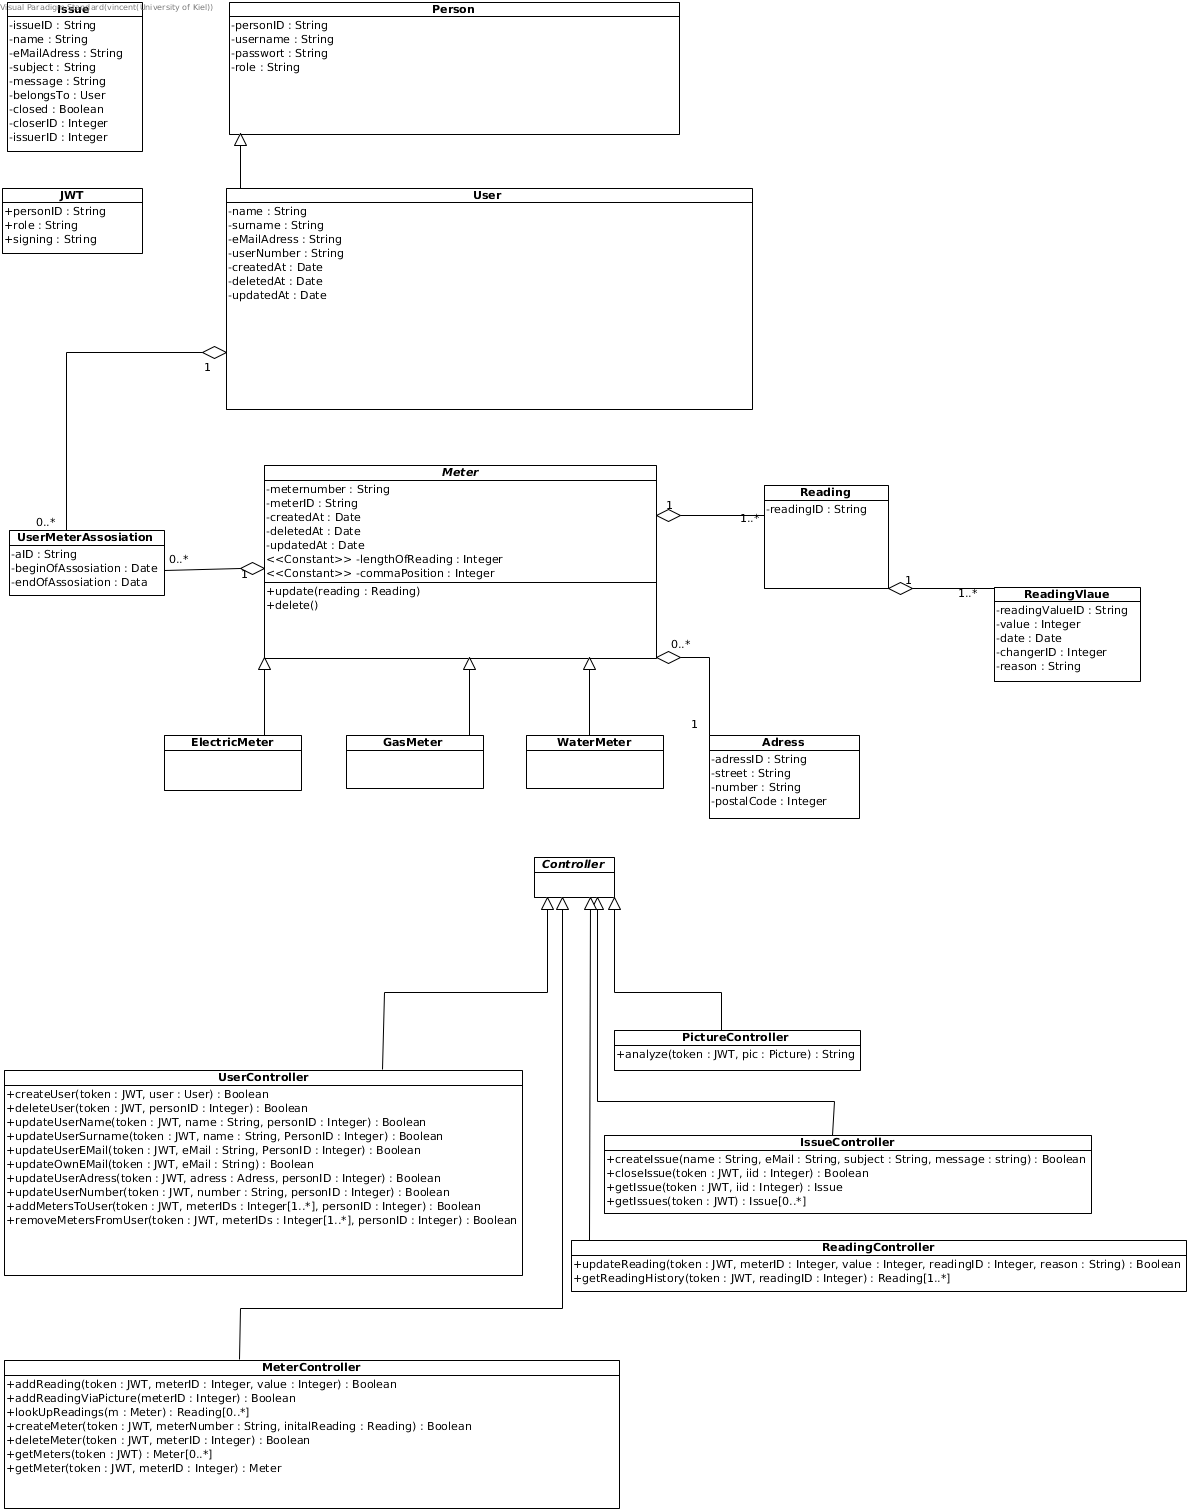
\includegraphics[width=15cm]{img/diagrams/backend-class-diagram}\\
\caption{Klassendiagramm - Back-End}
\end{figure}
Bei allen Objekten, die Entities des Models darstellen (Person, User, UserMeterAssociation, Meter, Reading, ReadingValue, Adress, Issue), handelt es sich um Spring Entity-Objekte.
Die normalerweise anfallenden Klassen (z.B. Repository-Klassen) werden zwar generiert, aber zu Übersichtszwecken nicht im Diagramm aufgeführt.\\
JWT steht für JSON Web Token. 
JWTs werden genutzt, um bei Anfragen an die REST-API User und Administratoren zu authentifizieren. Die REST-API wird durch den Controller bereitgestellt.
Man kann daher auch aus jeder Anfrage, die einen JWT enthält, einen konkreten User herauslesen. 
Da es sich um ein JSON-Objekt handelt, wird es intern nur als String wahrgenommen, aber zur Übersicht im Diagramm wurde es mit dem geplantem Inhalt als Java-Klasse aufgeführt.\\
Da Kunden aus einer Wohnung ausziehen können und neue Kunden dort einziehen können, benötigen Kunden und Zähler eine Komponente oder Funktion, welche einen Zähler zu einem Gewissen Zeitpunkt einem Kunden zuordnet. 
Zu diesem Zweck existiert die UserMeterAssosiation.\\
Ein Zähler besitzt mindestens einen aktuellen Zählerstand und gegebenenfalls mehrere alte Zählerstände, sowie eine Adresse, an der er montiert ist.\\
Das Attribut lengthOfReading wird von den konkreten Zählern geerbt und beschreibt, welche Länge eine Eingabe dieser Zählerart besitzt. Das Attribut commePosition besagt dabei, wie viele Nachkommastellen es gibt.\\
Ein Zählerstand hat mindestens einen Wert der beim Ablesen angegeben wird. 
Da er aber unter Umständen von Administratoren geändert werden kann, werden zusätzlich alle Versionen des Zählerstandes inklusive der Person die ihn verändert hat, ebenfalls wird der Grund für die Änderung gespeichert.
Beim Erstellen eines Zählerstandes wird ein ReadingValue aus dem tatsächlichen Stand des Zählers und Default-Werten für Grund und Ersteller generiert.\\
Die Controller dienen zum Auslesen und Manipulieren der Daten des Models. 
Die Controller sind jeweils darauf spezialisiert die Anfragen von Nutzern, Zählern oder Einträgen zu händeln.

\section{Klassendiagramme - App}
Die App ist intern in eine View- und eine Model/Controller-Komponente aufgeteilt. Es folgen Klassendiagramme für die 2 Komponenten.
\begin{figure}[H]
\centering
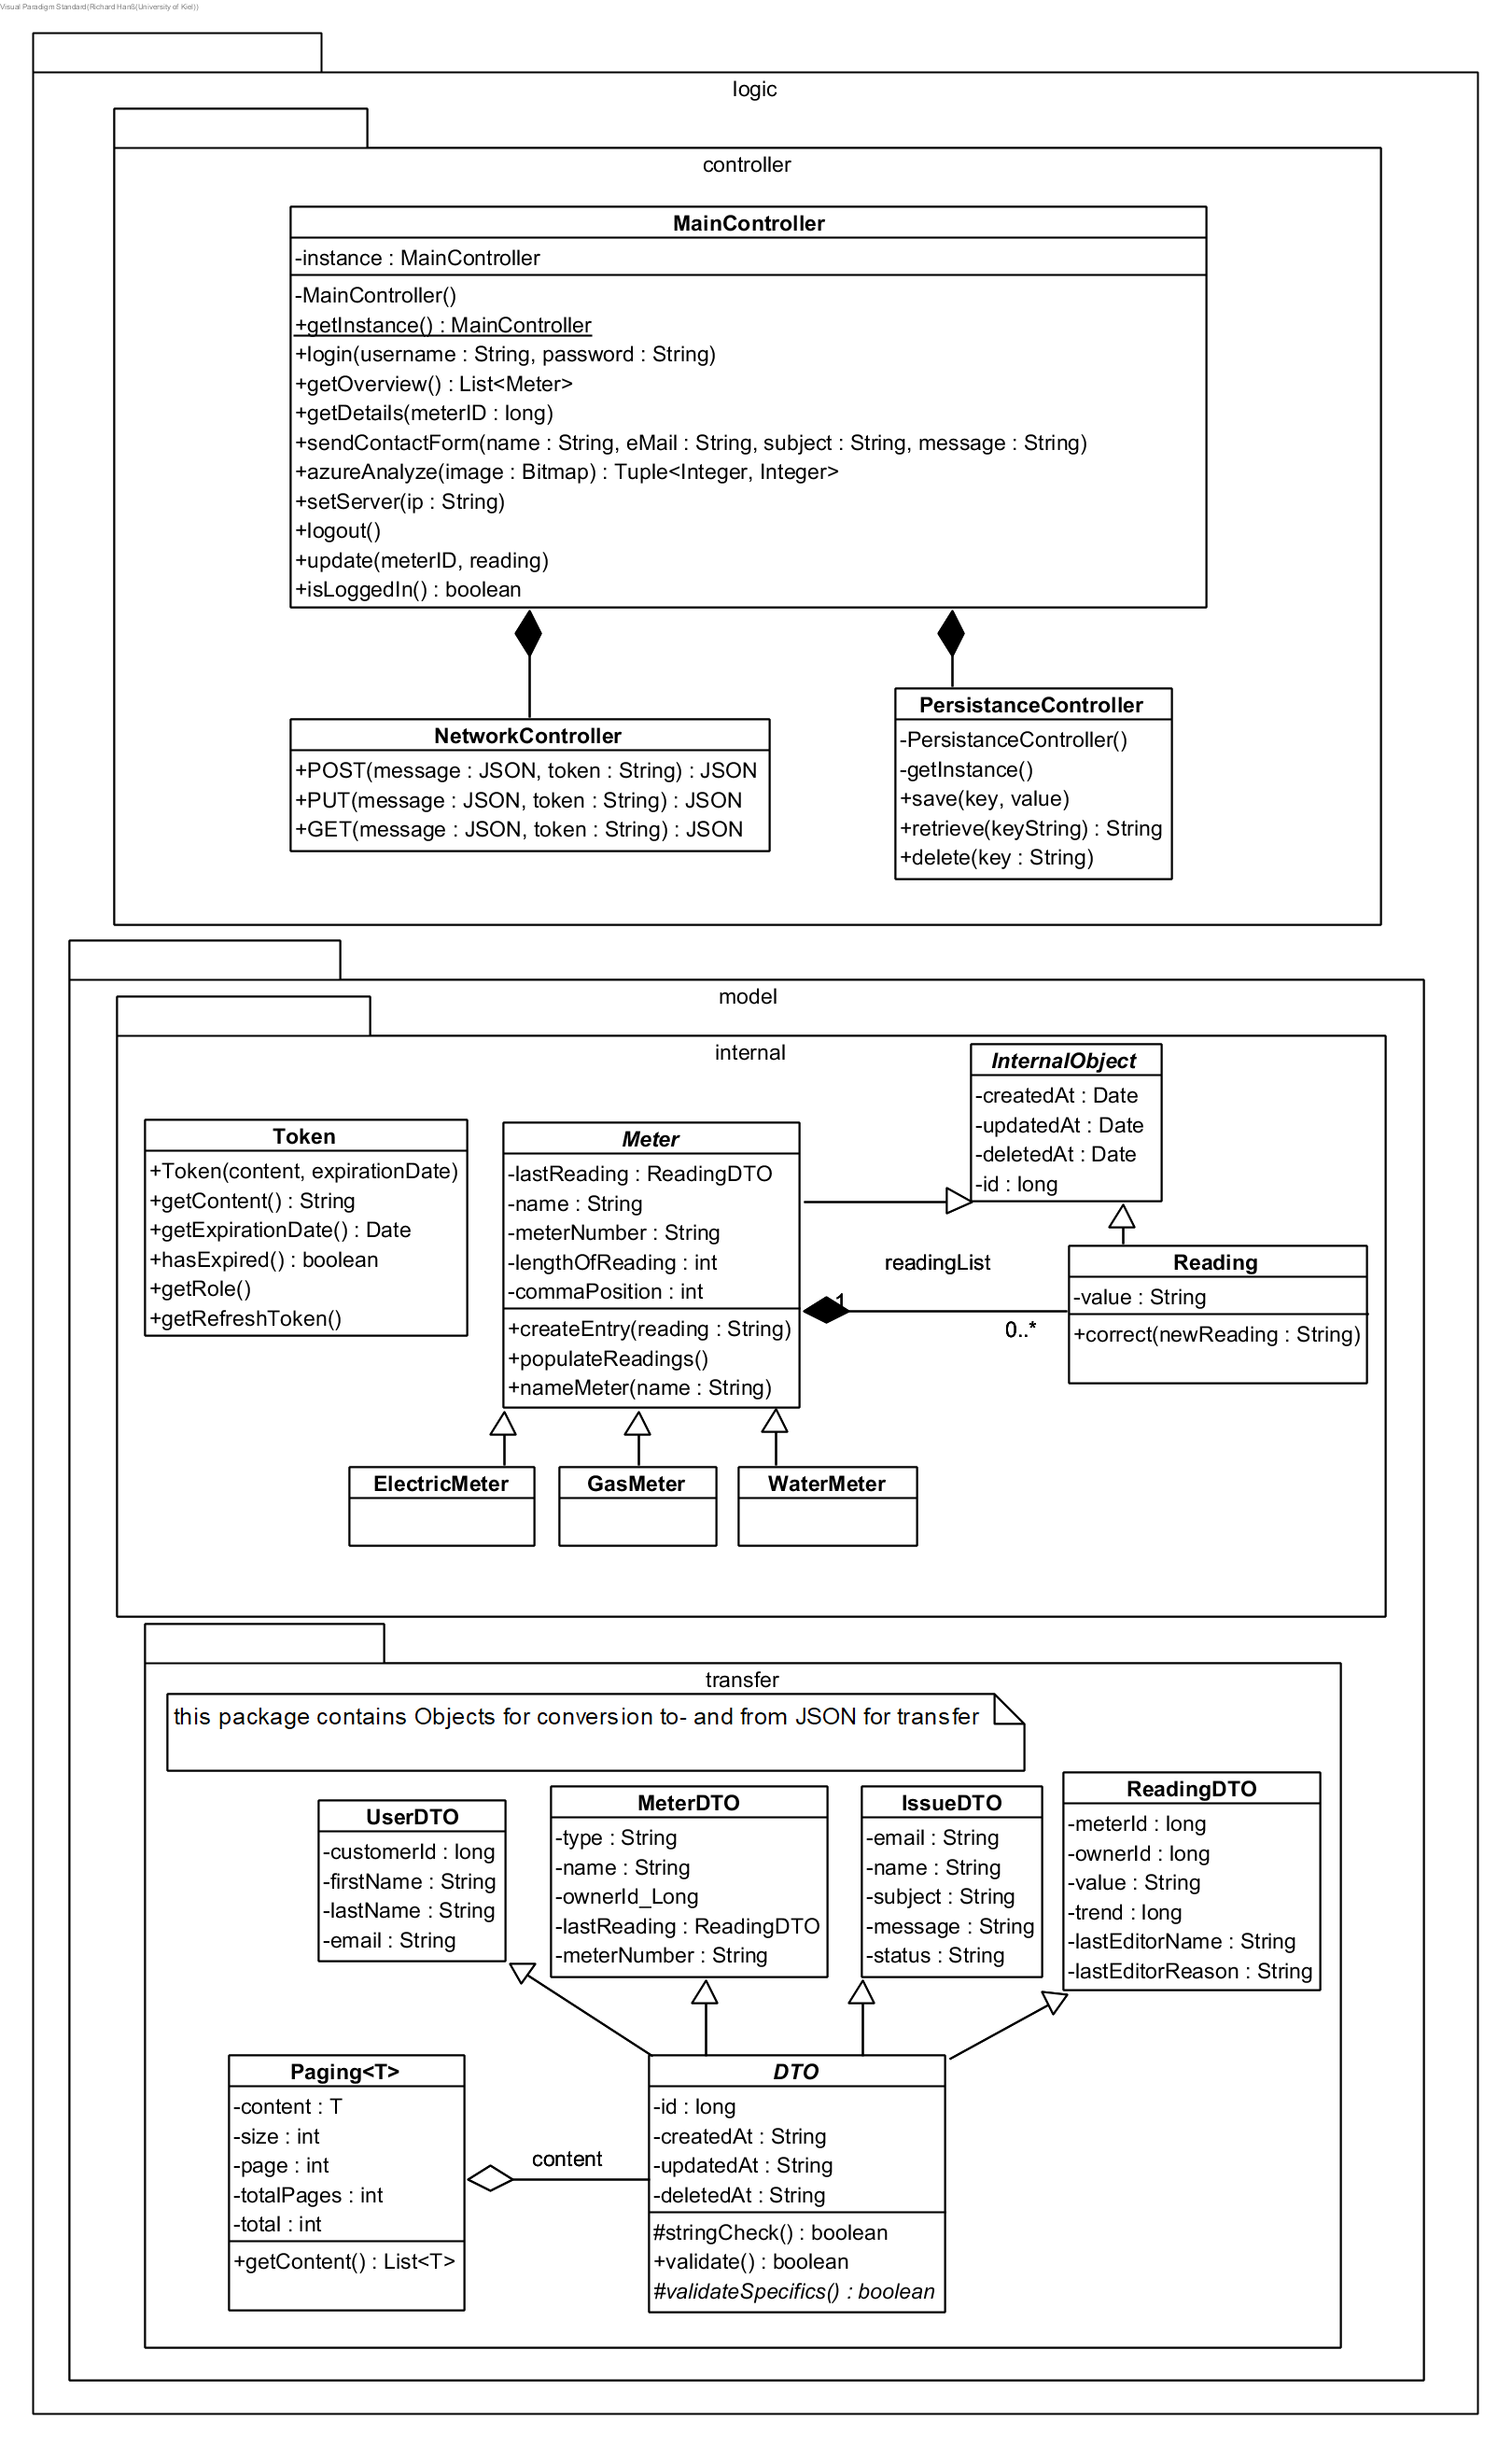
\includegraphics[height=20cm,width=15cm]{img/diagrams/Android-Class-Diagram-Logic}\\
\caption{Logik der App}
\end{figure}


\subsection*{Erklärung - Model \& Controller der App}
Im Package 'logic' befinden sich die Packages 'model' und 'controller'.
Klassen im Controller-Package sind verantwortlich fürs tatsächliche Ausführen der Operationen, die vom User über Interaktion mit den Views gestartet werden. \\ Die Singleton-Klasse MainController ist hier erster Ansprechpunkt für die Views und stellt Methoden zum Ein- und Ausloggen, Analysieren von Bildern, Fetchen von Zählern, Senden von Kontaktanfragen und ändern vom zu benutzendem Server. \\ Der MainController benutzt zum senden von HTTP-Requests den NetworkController und zum Speichern von persistenten Daten (wie z.b. OAuth Token) den PersistanceController.
Das Model ist in 2 Packages unterteilt. 'internal' enthält Objekte, die den Views zur Anzeige übergeben werden, sowie eine Repräsentation des OAuth-Tokens. \\ Im 'transfer' package befinden sich Klassen, die identisch zu den über REST zu übertragenden JSON Objekten aufgebaut sind. Sie werden über eine Library von- und zu JSON konvertiert werden.

\begin{figure}[H]
\hspace{-1cm}
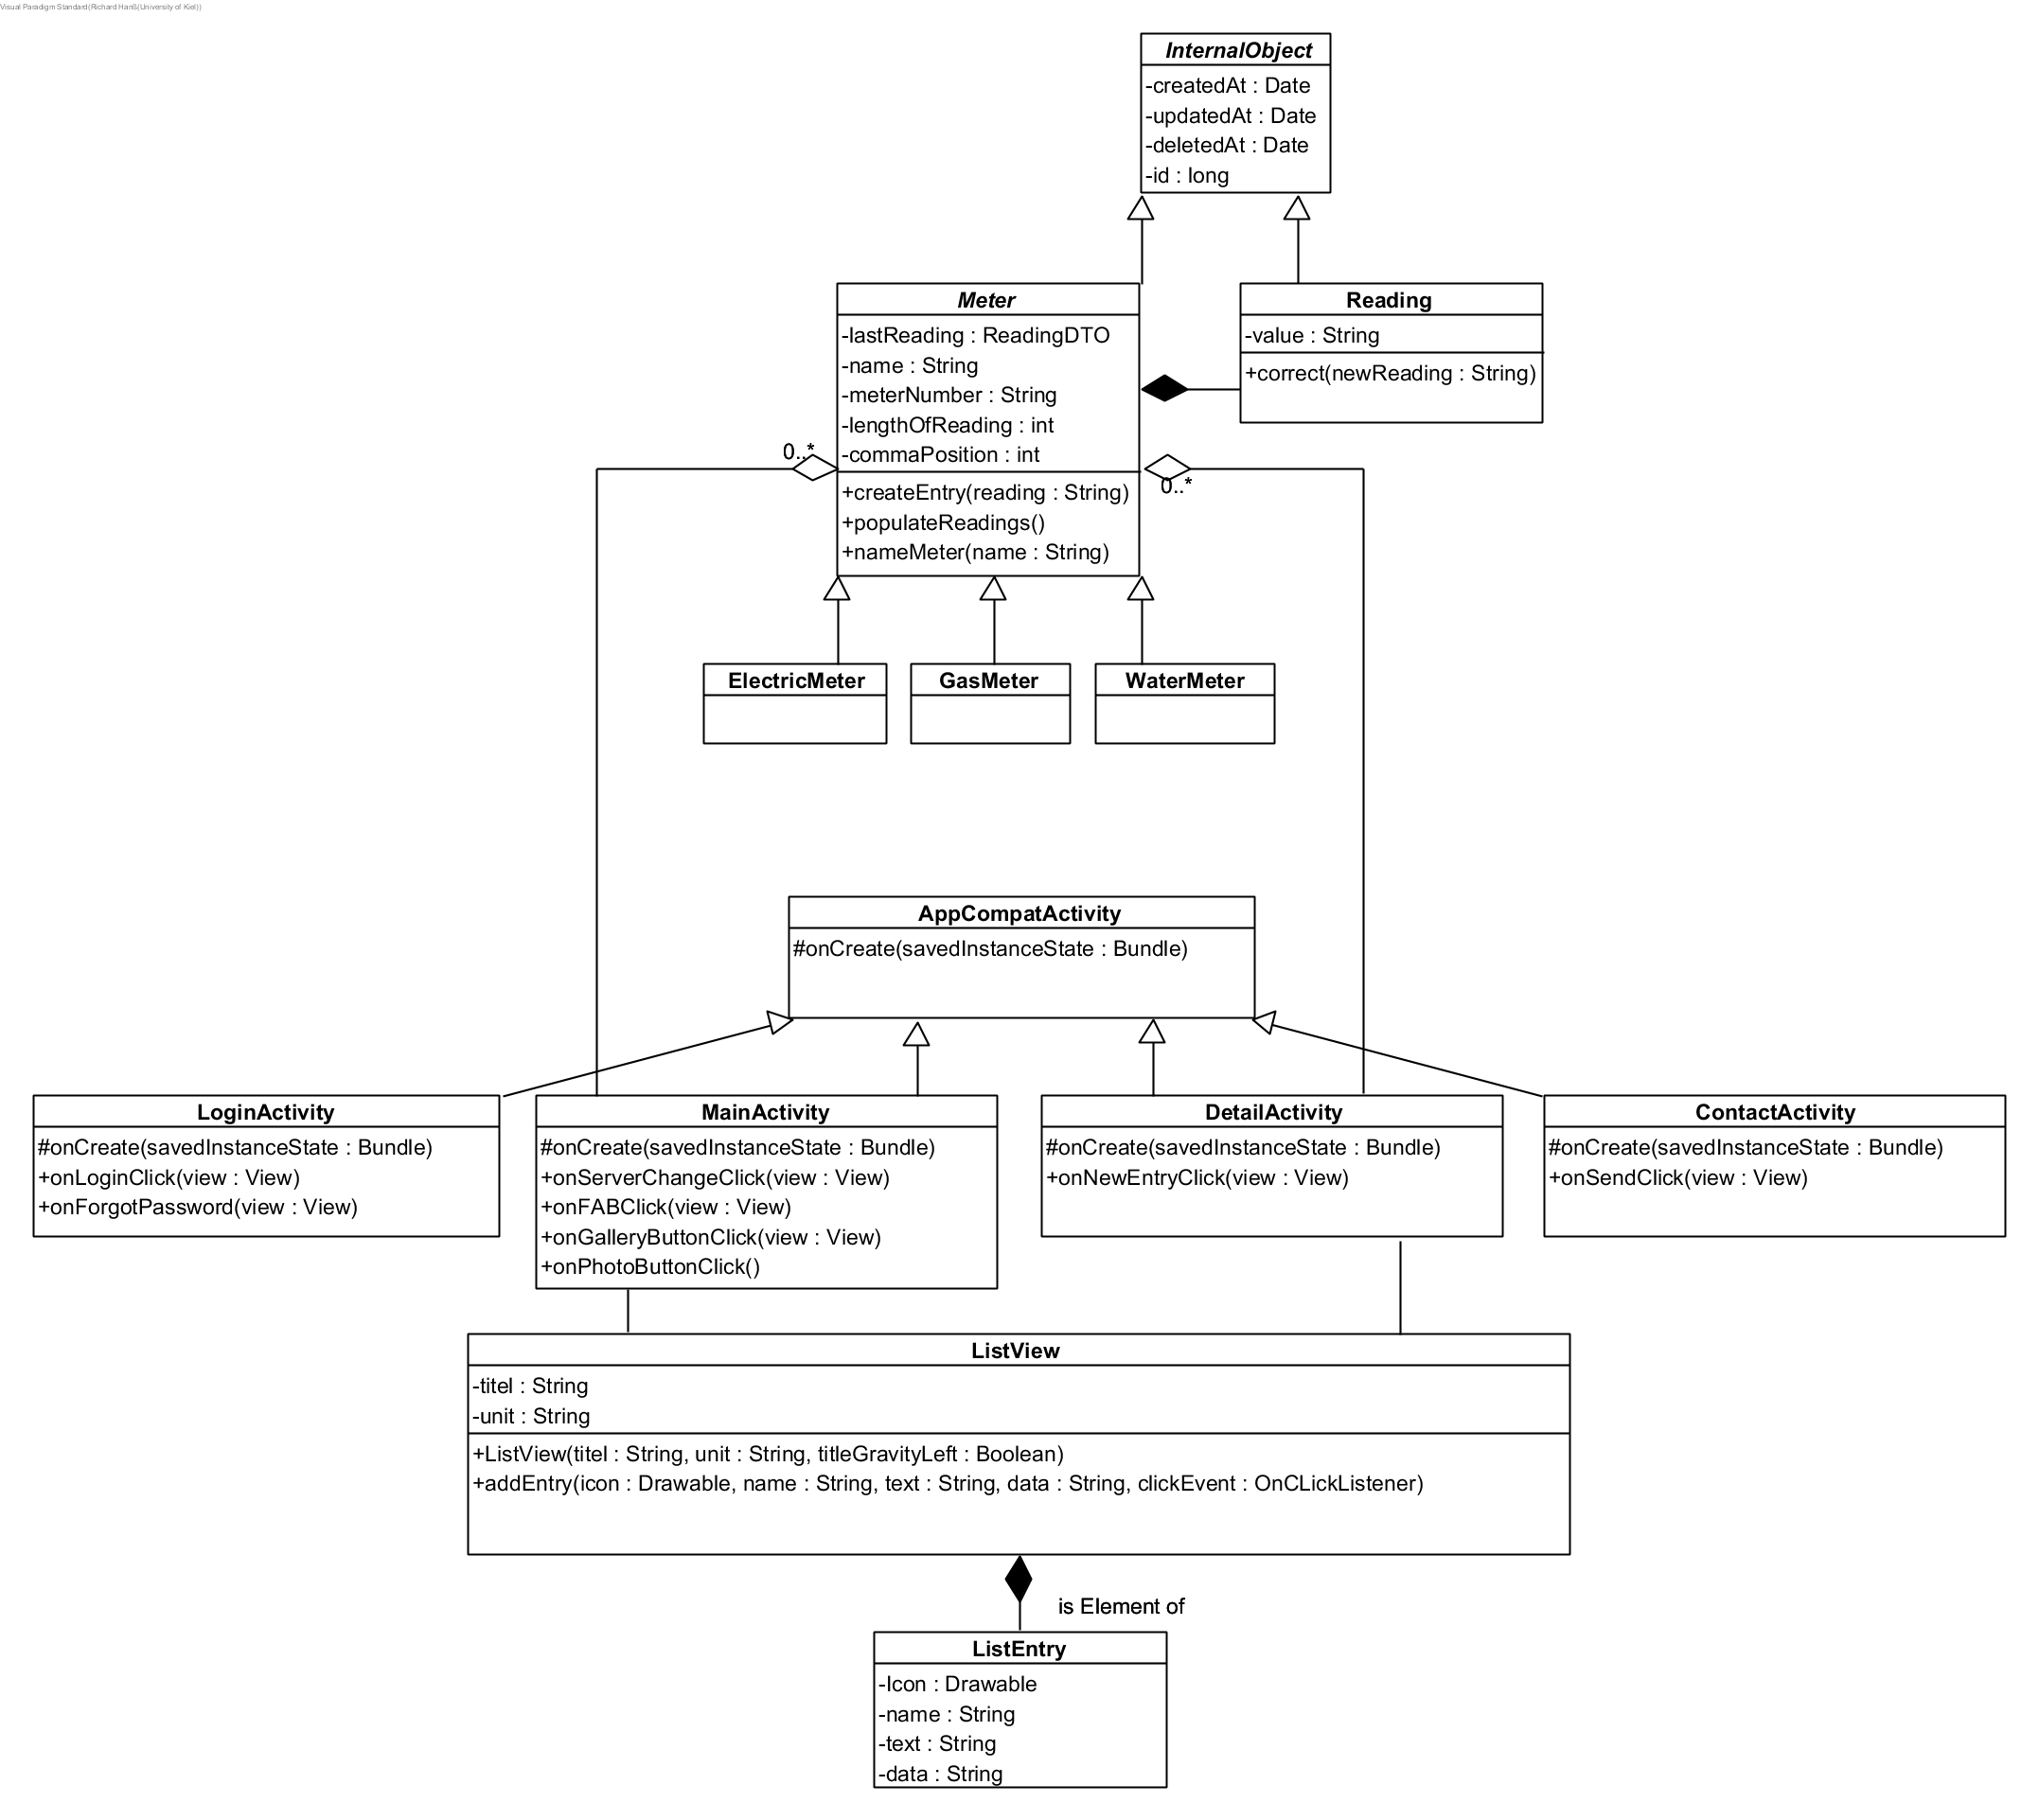
\includegraphics[height=14cm]{img/diagrams/Android-Class-Diagram-View}\\
\caption{Android View}
\end{figure}

\subsection*{Erklärung - View der App}
\begin{tabularx}{15cm}{XX}
	\hline
	Meter/InternalObject/Reading & Die hier aufgeführte Meter Klasse ist dieselbe, die auch in dem Logikdiagram dargestellt ist. \\ \hline
	ElectricMeter/GasMeter/WaterMeter & Die hier aufgeführte Meter Klasse ist dieselbe, die auch in dem Logikdiagram dargestellt ist. \\ \hline
	AppCompatActivity & Diese Klasse ist standartmäßig die Superklasse von allen Activities in Android Studio \\ \hline
	LoginActivity & Diese Activity stellt UI Elemente bereit, die es dem Nutzer erlauben sich anzumelden. \\ \hline
	MainActivity & Auf dieser Activity kann der Nutzer seine Zähler und einige Zählerstände einsehen, sowie auf sie zugreifen. \\ \hline
	DetailActivity & Auf dieser Activity kann der Nutzer Zählerstände hinzufügen und einsehen. \\ \hline
	IssueActivity & Auf dieser Activity kann der Nutzer einen Admin kontaktieren, falls er ein Problem hat. \\ \hline
	ListView & Diese Klasse erleichtert das hinzufügen und maintainen von Listen in der ManActivity und DetailActivity. \\ \hline
	ListEntry & Diese Klasse stellt einen Listeneintrag dar. 
\end{tabularx}
